\chapter{Forecasts}

WHAT DO THESE TERMS ALL HAVE IN COMMON: BREAKOUTS, Elliott waves, Fibonacci waves, \textbf{exponentially weighted moving average crossover} and Bollinger bands? Answer: They can all form the basis of \textbf{trading rules}. These rules give you \textbf{forecasts} of what they think will happen to the prices of \textbf{instruments} you are trading or investing in.

\textbf{Staunch systems traders} use multiple systematic rules like these. But rules can also be extremely simple, like the single rule used by \textbf{asset allocating investors}. It's also possible to use my \textbf{framework} without any systematic rules at all, as a \textbf{semi-automatic trader} making your own discretionary forecasts.

\section*{Chapter overview} \phantomsection \addcontentsline{toc}{section}{Chapter overview}

\begin{chapteroverviewtable}
\chapteroverviewitem{What makes a good forecast}{Understand the important properties of the forecasts which trading rules produce.}
\chapteroverviewitem{Discretionary trading with stop losses}{How semi-automatic traders can make forecasts that have the right characteristics.}
\chapteroverviewitem{The asset allocating investor's `no-rule' rule}{The simplest possible trading rule used by asset allocating investors -- a constant and identical forecast for all assets.}
\chapteroverviewitem{Two systematic rules}{A pair of suggested trading rules for staunch system traders.}
\chapteroverviewitem{Using other people's rules}{How to adapt publicly available trading rules or invent your own.}
\chapteroverviewitem{Selecting trading rules and variation}{A brief reminder of how I recommend selecting rules and variations.}
\end{chapteroverviewtable}

\section*{What makes a good forecast} \phantomsection \addcontentsline{toc}{section}{What makes a good forecast}

Parts of this section are quite technical; \textbf{semi-automatic} \textbf{traders} and \textbf{asset} allocating \textbf{investors} should read it but need only skim the content. However, \textbf{staunch systems traders} who will design their own trading rules need to understand it in detail.

\subsection*{A forecast is a scaled quantity}

When I started trading options at a large investment bank I was encouraged to put on small proprietary positions outside of the normal customer flow trading. The idea was to give novices some practical experience in managing risk without exposing the book to large losses. Initially I was limited to trading single futures contracts.

Once I graduated beyond one contract I was faced with a dilemma. How big should my position be for a purchase of German 10 year bond futures (Bunds)? Should I stick to one contract, or increase my size? I asked for advice from a more experienced trader, Sergei.\footnote{Not his real name.} He sighed, exasperated at the ignorance of youth, and turned towards me.

\begin{quote}
"You need to know three things. First, how much do you like this trade? That comes from here," Sergei replied, pointing to his heart. 

"Second thing, how much can you afford to lose? That is down here, in your gut," and he patted his extensive stomach. 

"Last thing, how risky is it? You calculate that here." said Sergei, tapping his forehead.
\end{quote}

His answer was unhelpful, completely lacking in any detail, but totally correct.

It's not enough to predict that prices are rising or falling; you also need to decide whether they will go up a lot, or a little. You need to decide how much you like the trade. You need a \textbf{forecast} -- a prediction of how much prices are expected to go up or down. This chapter is about making forecasts. I'll return to the rest of Sergei's wisdom in subsequent chapters.

A forecast is a number: a positive value means you want to buy the asset because the price is expected to go up and a negative indicates you want to short the asset. Investors who don't use derivatives and can't \textbf{short sell} will only make positive forecasts. A forecast shouldn't be binary -- buy or sell -- but should be scaled. Forecasts close to zero indicate a small movement in prices and larger absolute values mean you expect bigger returns.

There are three reasons why scaled forecasts make sense. Firstly, if you were to examine the returns made by a trading rule given the size of its forecasts, you'd normally find that forecasts closer to zero aren't as profitable as those further away. Secondly, binary systems cost more to trade, since to go from long to short you'd need to sell twice a full size position immediately. Finally, the rest of the framework assumes that the forecasts you get are not binary or lumpy in other ways.\footnote{Technical notes: There are two main reasons for this. Firstly, forecasts should have well defined and relatively stable \textbf{standard deviations}, otherwise the risk properties of the trading system will not be well defined or stable. Secondly, as we'll see subsequently I recommend limiting absolute forecast values to twice their average. Forecast distributions which are more extreme than \textbf{Gaussian normal distributions} will see an undesirable level of forecast capping. Note that there is a special case where lumpy or even binary forecasts will work just fine. If we have a large number of relatively uncorrelated binary forecasts then once combined these will approach a desirable Gaussian normal.} It's better to see forecasts changing continuously rather than jumping around.

It's relatively easy to design or adapt a trading rule to produce scaled forecasts, if you're a \textbf{staunch systems trader}. If you're a \textbf{semi-automatic trader} generating forecasts in a more discretionary way then you need to be able to quantify the strength of your convictions and I'll return to that problem later in this chapter. \textbf{Asset allocating investors} have it easy since they use a fixed forecast value.

\subsection*{Forecasts proportional to risk adjusted return}

How do you set forecasts so that they embody how much you like a position, or to be precise how strong you think its subsequent rise or fall will be?

Simple, you might think. As I was trading Bunds when I spoke to Sergei then I should set up my \textbf{trading rule} so a weak forecast of 50 would mean a purchase of 50 Bund futures. A strong forecast of 100 implies 100 contracts, and so on.

Unfortunately there are several flaws in this idea. What if you wanted to use my forecasting rule? You might not want to take a gamble on even five Bunds, or you could work in a large fund for whom an average position would be 50,000 contracts. This kind of forecast doesn't account for different account sizes or varying appetite for risk.

Secondly, what if the \textbf{standard deviation} of Bund prices were to double? A position of 50 contracts would now be twice as risky as you'd originally expected. The simple forecast doesn't account for risk changing over time.

Finally, you'd normally want to use the same trading rule across different \textbf{instruments}, because it's simpler and it allows you to pool data if you're \textbf{fitting}. However 50 Bunds expose you to much less risk than 50 Japanese government ten year bond futures, but to much more than 50 German Schatz (two year) bond futures. The rule can't cope with instruments which don't have the same risk.

The solution is to use my favourite technique, \textbf{volatility standardisation}. So in my framework forecasts are proportional to expected risk adjusted returns. For example suppose that the Bund has expected returns of 2\% a year and an expected annualised standard deviation of 8\%. Schatz futures have an expected return of 1\% a year, but you only expect \textbf{volatility} of 2\% a year. After adjusting for risk the expected return on Schatz (1\% ÷ 2\% = 0.5) is twice as much as on Bunds (2\% ÷ 8\% = 0.25).

That implies the forecast for Schatz should be twice the forecast for Bunds. This deals with instruments that have different risks. It also means any trading rule can be used without modification on all instruments and that if you fit trading rules you can do so with pooled data from multiple assets. If you continuously adjust your estimate of expected volatility then you also cope with risk changing over time.

Finally with forecasts like these different investors can use the same trading rules, but then scale positions depending on the size of their accounts and their appetite for risk. I show how this is done in chapter nine, ‘Volatility targeting', and chapter ten, ‘Position sizing'. 

You've seen before that the ratio of average return to standard deviation of returns is the \textbf{Sharpe ratio}. So expected Sharpe ratios make good forecasts, which makes creating trading rules very intuitive.

\subsection*{Forecasts should have a consistent scale}

I said above that a forecast needs to be proportional to the risk adjusted return. In the example above forecasts of 2.5 for Bunds and 5 on Schatz; 0.0000005 and 0.000001 respectively, or 5,000 and 10,000, are all valid. Which of these, or the infinity of other options, is best?

In truth it doesn't really matter, as long as you are consistent, but whichever scaling you choose here will affect the rest of your trading system. In particular the expected average absolute value of your forecasts is a key part of specifying the system. Life will be easier if you choose a scaling that is easy to work with. Very small or large numbers are difficult for humans to cope with and even computers struggle with floating point representation of tiny fractions.

My recommendation is to create forecasts which have an expected absolute value of 10. So +10 is an average buy and -10 an average sell. A forecast of +5 would be a weak buy, and -20 is a very strong sell. These forecast numbers may seem very abstract right now. Don't be too concerned as in chapter ten ‘Position Sizing' I will show you how to translate them into actual positions.

If you're a \textbf{semi-automatic trader} using discretionary forecasts, it's straightforward to have the right scaling, as I will show you below. The rule used by \textbf{asset allocating investors} also has the appropriate scale. The example rules I provide for \textbf{staunch systems} traders later in the chapter are also correctly scaled. But if you're making your own rules, or adapting others, you will need to standardise their natural scaling, as I'll explain later in the chapter.

\subsection*{Should we allow forecasts to be as large as possible?}

With an expected absolute value of 10, a forecast of +10 is bullish, and one of +20 is really bullish. What if you're confident that this is the chance of a lifetime, like the 2009 Barclays trade which I told you about in the introduction. Should you allow your rule to have a forecast of +100? I think not. Forecasts should be capped at a maximum absolute value and I recommend a limit of 20. Here's why:

\begingroup
\small
\setlength{\tabcolsep}{5pt}
\renewcommand{\arraystretch}{1.12}
\noindent\begin{breakabletabularx}{\textwidth}{@{} L{0.21\textwidth} Y@{}}
\toprule
\endfirsthead
\toprule
\endhead
\bottomrule
\endfoot
\bottomrule
\endlastfoot
\shortstack[l]{\textbf{Risk control}} & Diversification is the investor's best friend. But it's pointless diversifying if you then allow one part of your system to dominate your returns. You need to limit the risk that any trading rule variation can contribute to the overall system. \\
\midrule
\shortstack[l]{\textbf{Limited data}} & When I back-test a profitable trading rule I normally find that positive forecasts are associated with price rises, and larger values mean larger rises. However for a properly scaled rule very large forecast values will appear rarely in a back-test. So there is a lot of uncertainty around whether extremely large forecasts translate into proportionally larger price movements, as I don't usually have enough data to support this finding.\par
If a forecast had a Gaussian normal distribution you'd only see absolute forecast values over 20 around 5\% of the time, so there is only limited evidence that forecasts of this magnitude are actually correct. \\
\midrule
\shortstack[l]{\textbf{Extremes are}\\ \textbf{often different}} & Normally markets trend with falls followed by further falls, but after very sharp drops subsequent one day rises are more likely; the so called ``dead cat bounce''. Similarly high yielding stocks do well, but those with dividend yields above 50\% are probably going bankrupt, or at the very least about to cut their dividend. Many other patterns also reverse at extremes. These effects are not often strong or common enough to exploit directly, but they should give you concern about betting too much when you have very strong forecasts. \\
\midrule
\shortstack[l]{\textbf{Higher realised}\\ \textbf{return volatility}} & A high forecast could mean that you expect large returns, but equally it might be due to very low standard deviation of returns. Unfortunately periods of subdued volatility are usually followed by jumps to much higher levels, often combined with reversals in price.\par
I had very strong positive forecasts in the Japanese Bond markets in January 2013, mainly due to relatively low volatility. When Prime Minister Abe unveiled his latest set of economic reforms volatility spiked rapidly as prices dropped fast. Fortunately because my forecasts were capped the damage was contained. \\
\midrule
\shortstack[l]{\textbf{Limited}\\ \textbf{downside}} & If forecasts have a Gaussian normal distribution then it's rare, again around 5\% of the time, that you'll see values bigger than 20. So the reduction in your returns from capping is quite small compared to the potential risk control benefits. \\
\end{breakabletabularx}
\endgroup

Staunch systems traders shouldn't ignore forecasts that are outside of the range -20 to+20, but cap them. A forecast of +25 from your trading rule should be reduced to +20. Increase any forecast lower than -20 to that level. All your forecasts will then be in the range -20 to +20.

For \textbf{semi-automatic traders} all your discretionary forecasts should be in the range of-20 to +20, with no exceptions, even for the trade of a lifetime. \textbf{Asset allocating investors} don't need to worry as you will have a fixed forecast of +10.

If we can't short an instrument, because of limited access to derivatives or difficulties \textbf{selling short}, then you'll also need to change all negative forecasts to zero.

\section*{Discretionary trading with stop losses} \phantomsection \addcontentsline{toc}{section}{Discretionary trading with stop losses}

\subsection*{Semi-automatic Trader}

If you're a \textbf{semi-automatic trader} then you won't use systematic trading rules but instead make \textbf{discretionary} forecasts either on gut feeling, or using complex analysis which can't be systematised, like my 2009 Barclays trade in the introduction. As well as the sign of the forecast, positive for long and negative for short, you must indicate how strongly you feel about it. Your forecasts must be correctly scaled: the expected absolute value should be around 10, and they must be between the recommended limits of -20 and +20.

Forecasts don't have to be finely quantified, such as "I love the Nikkei today, about 8.7663." However, you should be able to give a rough indication of the strength of your passion for the Nikkei. You can then translate your opinion into a forecast number, as table 16 shows.

\rawtablecaption{TRANSLATING OPINIONS INTO A QUANTIFIED FORECAST} \begingroup \small \setlength{\tabcolsep}{2pt} \renewcommand{\arraystretch}{1.15} \begin{tabularx}{\textwidth}{@{}*{9}{>{\centering\arraybackslash} X}@{}}
\toprule
\shortstack{Very\\strong\\sell} & \shortstack{Strong\\sell} & Sell & \shortstack{Weak\\sell} & Neutral & \shortstack{Weak\\buy} & Buy & \shortstack{Strong\\buy} & \shortstack{Very\\strong\\buy} \\
\midrule
-20 & -15 & -10 & -5 & 0 & 5 & 10 & 15 & 20 \\
\bottomrule
\end{tabularx}
\endgroup

If you can’t go short assets, because you’re not using derivatives like spread bets or can’t \textbf{short sell} in your account, then you’ll need to limit yourself to positive forecast values. You shouldn’t change your forecast once a bet is open. Otherwise there is the risk of meddling, taking profits too early by reducing the conviction of your forecast or doubling up on a loss. Instead you will be using a systematic trailing stop loss rule to close all your positions. I’ll explain this further in chapter thirteen, where I describe a semi-automatic trading system in more detail. There are substantial advantages to using discretionary forecasts in my systematic framework with stop losses; you can make predictions about the behaviour of your live trading and measure expected risk more precisely. Your positions will always be the correct size for a given forecast, tolerance for risk, and account size. This will give you more time and energy to get the forecast right. Finally, by using stop losses you’ll be trading somewhat like an ‘early loss taking’ \textbf{trend follower}, so it’s more likely your strategy will have benign positive skew.

\section*{The asset allocating investor’s ‘no-rule’ rule} \phantomsection \addcontentsline{toc}{section}{The asset allocating investor’s ‘no-rule’ rule}

\subsection*{Asset Allocating Investor}

Think about a \textbf{static} portfolio of two \textbf{collective funds}: an S\&P 500 equity and a US benchmark bond fund. Suppose you bought them in equal weights, with half your cash in each. As bond funds tend to have a quarter of the \textbf{volatility} of equities this portfolio will have 80\% of its risk coming from stocks. As I explained in chapter two the solution is to hold the two assets in \textbf{risk parity}, each contributing the same amount of expected risk. This implies a cash weight to equities of roughly 20\% and 80\% to bonds.

By using the \textbf{framework}, instruments will automatically have identical expected standard deviation of returns for a given forecast level. This means if you have an equally weighted portfolio of two \textbf{trading subsystems}, one for equities and one for bonds, each with identical forecasts for their individual instrument, then you'd always have the same expected volatility for both equities and bonds. You'd effectively have a risk parity strategy where risk was being constantly adjusted, or what I described in chapter two as a ‘fourth degree' static portfolio (page 38).

Hence the correct rule for an \textbf{asset allocating investor} is to have a constant forecast equal to the expected average forecast, +10 for all instruments at all times. I call this the ‘no-rule' rule. You don't think you can predict how different assets will perform, so you buy them all. Remember all forecasts are proportional to return adjusted for standard deviation. So using an equal forecast for all instruments is equivalent to assuming all assets have the same expected \textbf{Sharpe ratio}.

There are certain advantages to using this constant forecast approach within the systematic framework, rather than just buying a normal risk parity portfolio. For starters you can probably do better than equal weights, as you will remember from chapter four, ‘Portfolio allocation'. Secondly, many risk parity funds don't adjust for the standard deviation of returns changing over time, whereas you will.\footnote{As you might recall from chapter two, page 38, many risk parity portfolios are ‘third degree’ with allocations set with initial expected risk, rather than the ‘fourth degree’ you will have (allocations adjusted as risk changes).} As I'll discuss in chapter twelve, ‘Speed and Size', that adjustment will be done after carefully considering the trading costs of our instruments. A DIY risk parity portfolio avoids paying the management fees you'd have with an external fund manager.

Finally, if you do decide to introduce expectations of asset returns there is a neat and relatively robust way to do this, by adjusting \textbf{handcrafted} portfolio weights in line with where you think prices will go. I'll give you more detail in the \textbf{asset allocating investor} example in part four of the book.

\section*{Two example systematic rules} \phantomsection \addcontentsline{toc}{section}{Two example systematic rules}

\subsection*{Staunch Systems Trader}

Semi-automatic traders and \textbf{asset allocating investors} can skip the remainder of this chapter, which is for \textbf{staunch systems traders} only. The two examples of \textbf{trading rules} above aren't very interesting. I include them to show how my framework can still be used by people who don't believe that market returns can be forecasted, or others who think they can do it better than a simple rule can. However staunch systematic traders disagree with both of these groups and wish to forecast prices with fully systematic trading rules.

There isn't enough space in this book to include every trading rule in existence. Fortunately, there's a plethora of other books and websites available which contain explicit trading rules, or ideas from which they can be developed. Just one book, Perry Kaufman's Trading Systems and Methods has over 1000 pages and includes dozens of rules.\footnote{There is a brief selection including this and other books in appendix A.} The next section in this chapter will show how you can create your own trading rules, or modify other people's.

In this section I will briefly outline two rules that I use in my own trading system.\footnote{Although these two rules represent only part of my trading system these two rules alone would account for around 85\% of back-tested performance. Unfortunately I'm unable to give a full description of every rule I use, partly because of space and also due to legal constraints.} If you want to use them you can find more detail in appendix B. In part four of this book I'll show how these rules can be incorporated into the framework to create a complete system for the staunch systems trader.

\subsection*{Trend following with the EWMAC rule}

Many asset prices seem to show \textbf{momentum}: what goes up, usually carries on going up; and vice versa. This effect can be captured by using \textbf{trend following} rules. I am a big fan of these types of rules for several reasons. Firstly, they work. As we saw in chapter one, the trend following ‘early loss taker' rule made mincemeat of its opposition, the ‘early profit taker'. There's a lot of academic research and real performance statistics supporting the use of trend following rules. Secondly, I like rules which I can explain; as I said in chapter two prospect theory justifies why these rules work, and should continue to do so. Also, trend following is an easy to implement technical strategy using only price data. Finally, it has benign positive skew.

Of course you could use the now familiar early loss taker rule for trend following, but there are better alternatives.\footnote{Early loss taker has some unpleasant attributes. First of all it gives a binary forecast; you are either long or short. Secondly, your current forecast depends on prices but also what positions you have recently had. This isn't a very nice property; amongst other things it means your precise \textbf{back-tested} behaviour will depend on where your price history began.} One of the most popular trading rules for capturing trends goes by the unwieldy name of \textbf{Exponentially Weighted Moving Average Crossover}, or EWMAC for short.\footnote{This is probably one of the oldest purely systematic trading rules in current use; ignoring the older, more subjective, technical analysis pattern matching tradition. There are academic studies of EWMAC dating back to the 1960s and it would have been used by traders prior to that.} Fortunately the idea is simpler to implement than it is to say. You take two \textbf{exponentially weighted moving averages (EWMA)} of an asset's price. One average, the slower, looks back over a longer period than the faster average. When the faster is above the slower it means that prices are in an uptrend and you should buy; and vice versa.

\begin{figure}[htbp] \centering 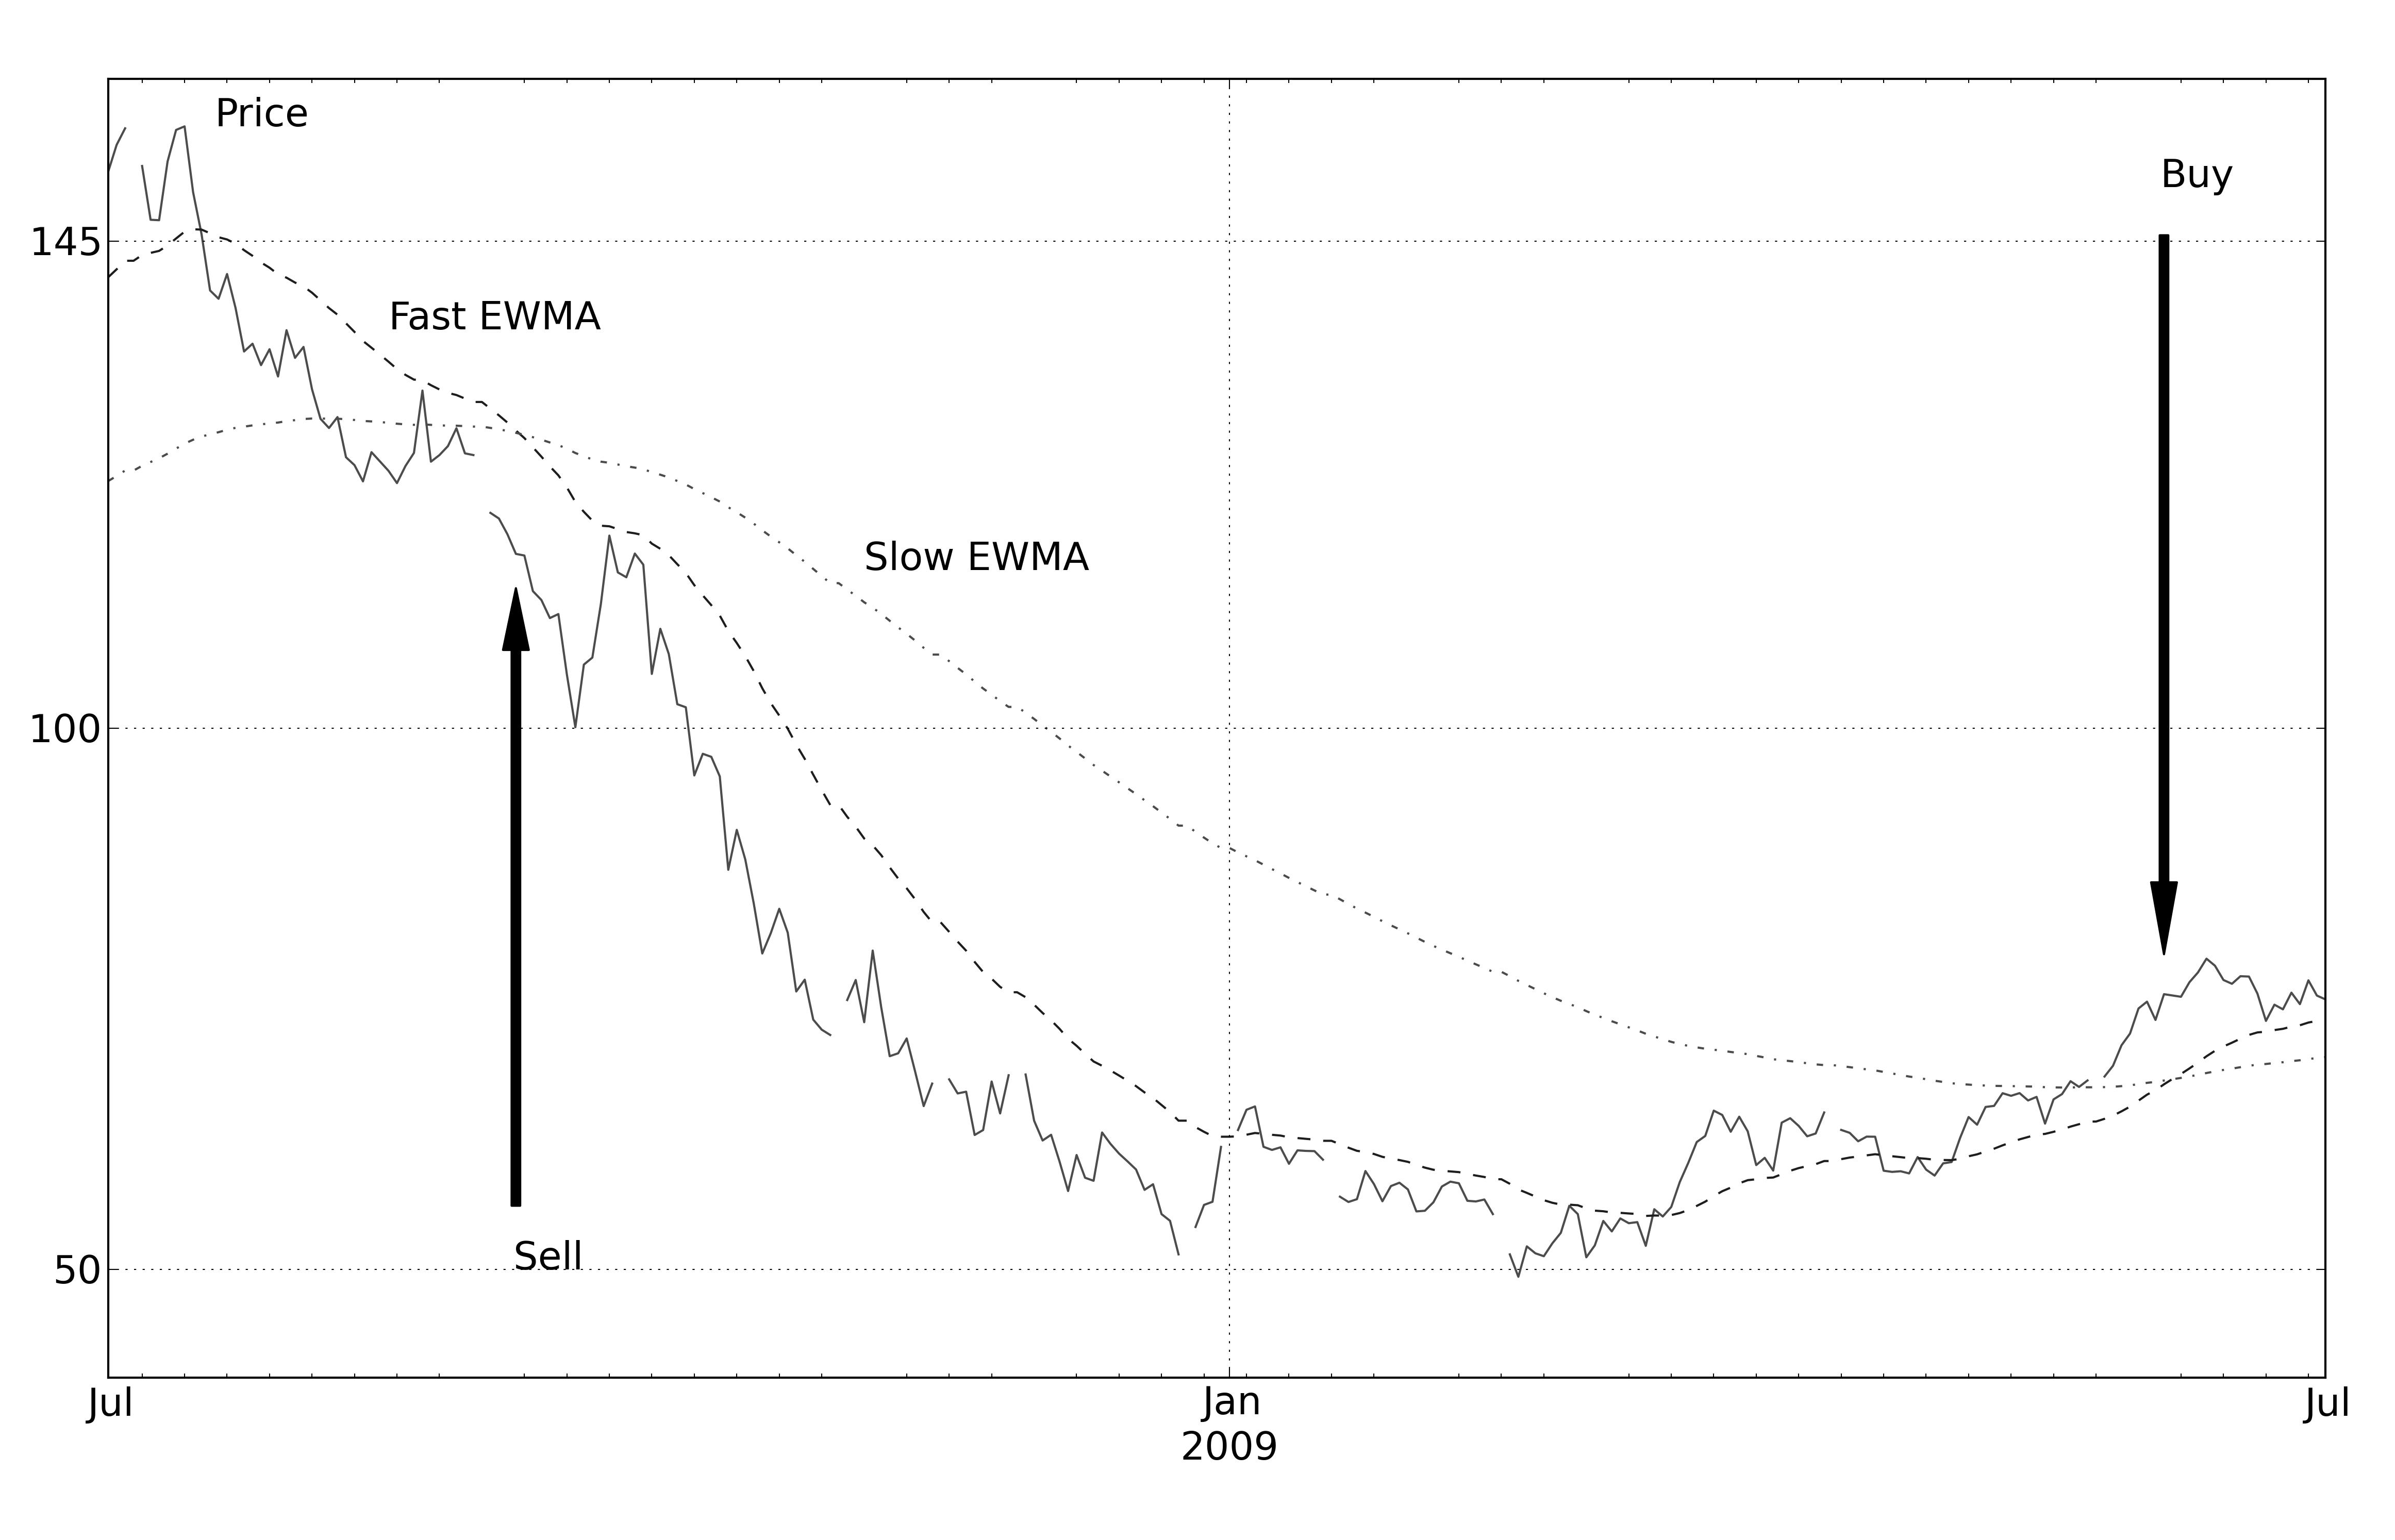
\includegraphics[width=\textwidth]{figures/raw/img-018.png} \caption{RIDING THE DOWNTREND IN CRUDE OIL FUTURES WITH THE EWMAC TREND FOLLOWING RULE. WE SELL WHEN THE FAST EWMA CROSSES THE SLOW; AND BUY WHEN THIS REVERSES} \end{figure}

Figure 18 shows an example. Here we've got the price of crude oil futures from summer 2008 onwards. After a long uptrend in prices there is a reversal in July 2008. Within a few weeks the fast EWMA has gone below the slower and goes short. The gap gets bigger and the position is increased until January. A gentle bullish trend begins and the short

is reduced, and then reversed once the fast EWMA climbs back above the slow in June

\begin{enumerate}
\item There is a detailed specification of the EWMAC rule in appendix B. \end{enumerate}

\subsection*{The carry rule}

EWMAC is a positive skew rule which needs prices to trend in one direction or another. To balance it out here is the \textbf{carry} rule which benefits when nothing happens. \textbf{Foreign} exchange carry is a well known strategy for exploiting stable markets; if you borrow in Japanese yen at 0.5\% and invest the money in Australian dollars at 3.5\% then you'll earn 3\%, assuming that the JPY/AUD exchange rate doesn't budge. But what does carry mean for other assets?\footnote{The first multi asset (rather than FX specific) academic research into carry appears to be the imaginatively titled working paper ‘Carry' by Ralph Koijen, Tobias Moskowitz, Lasse Pedersen and Evert Vrugt from 2012. The specification of the carry rule here is identical to that paper. But rules like this have been used in the industry for much longer.}

Carry, which is sometimes called roll down or contango, is the return that you will get if asset prices are perfectly stable. If the world doesn't change this will be equal to the yield on the asset, less the cost of borrowing (or the interest you would have got from holding cash). So if you buy shares in French supermarket Carrefour which currently has a dividend yield of 3\%, and you pay 1\% to borrow the purchase cost, then you earn 2\% carry on the position if the share price is unchanged.

Similarly today I can buy June 2018 Eurodollar futures at 97.94, or March 2018 at 98.01. If there is no change in the shape of the yield curve then in three months' time June futures will rise to 98.01, earning 0.07 per contract.

Academic theory predicts that prices should move against us to offset these returns, but it often doesn't. Carry is usually earned steadily on these kinds of trades although occasionally they go horribly wrong and the relationship temporarily breaks down, giving this trading rule some evil negative skew. I think the rule is profitable as a reward for taking on this nasty skew and various other kinds of \textbf{risk premium} which tend to be correlated to carry trades.

Full details on how I calculate carry are given in appendix B, from page 285 onwards. There is an example of the carry trading rule in action in figure 19, again showing crude oil futures during the great crash of 2008. The price of the nearer futures contract dips below the contract we are trading in mid-August. This is a bearish carry signal and the rule sells to enjoy some of the continuing fall in price.

\begin{figure}[htbp] \centering 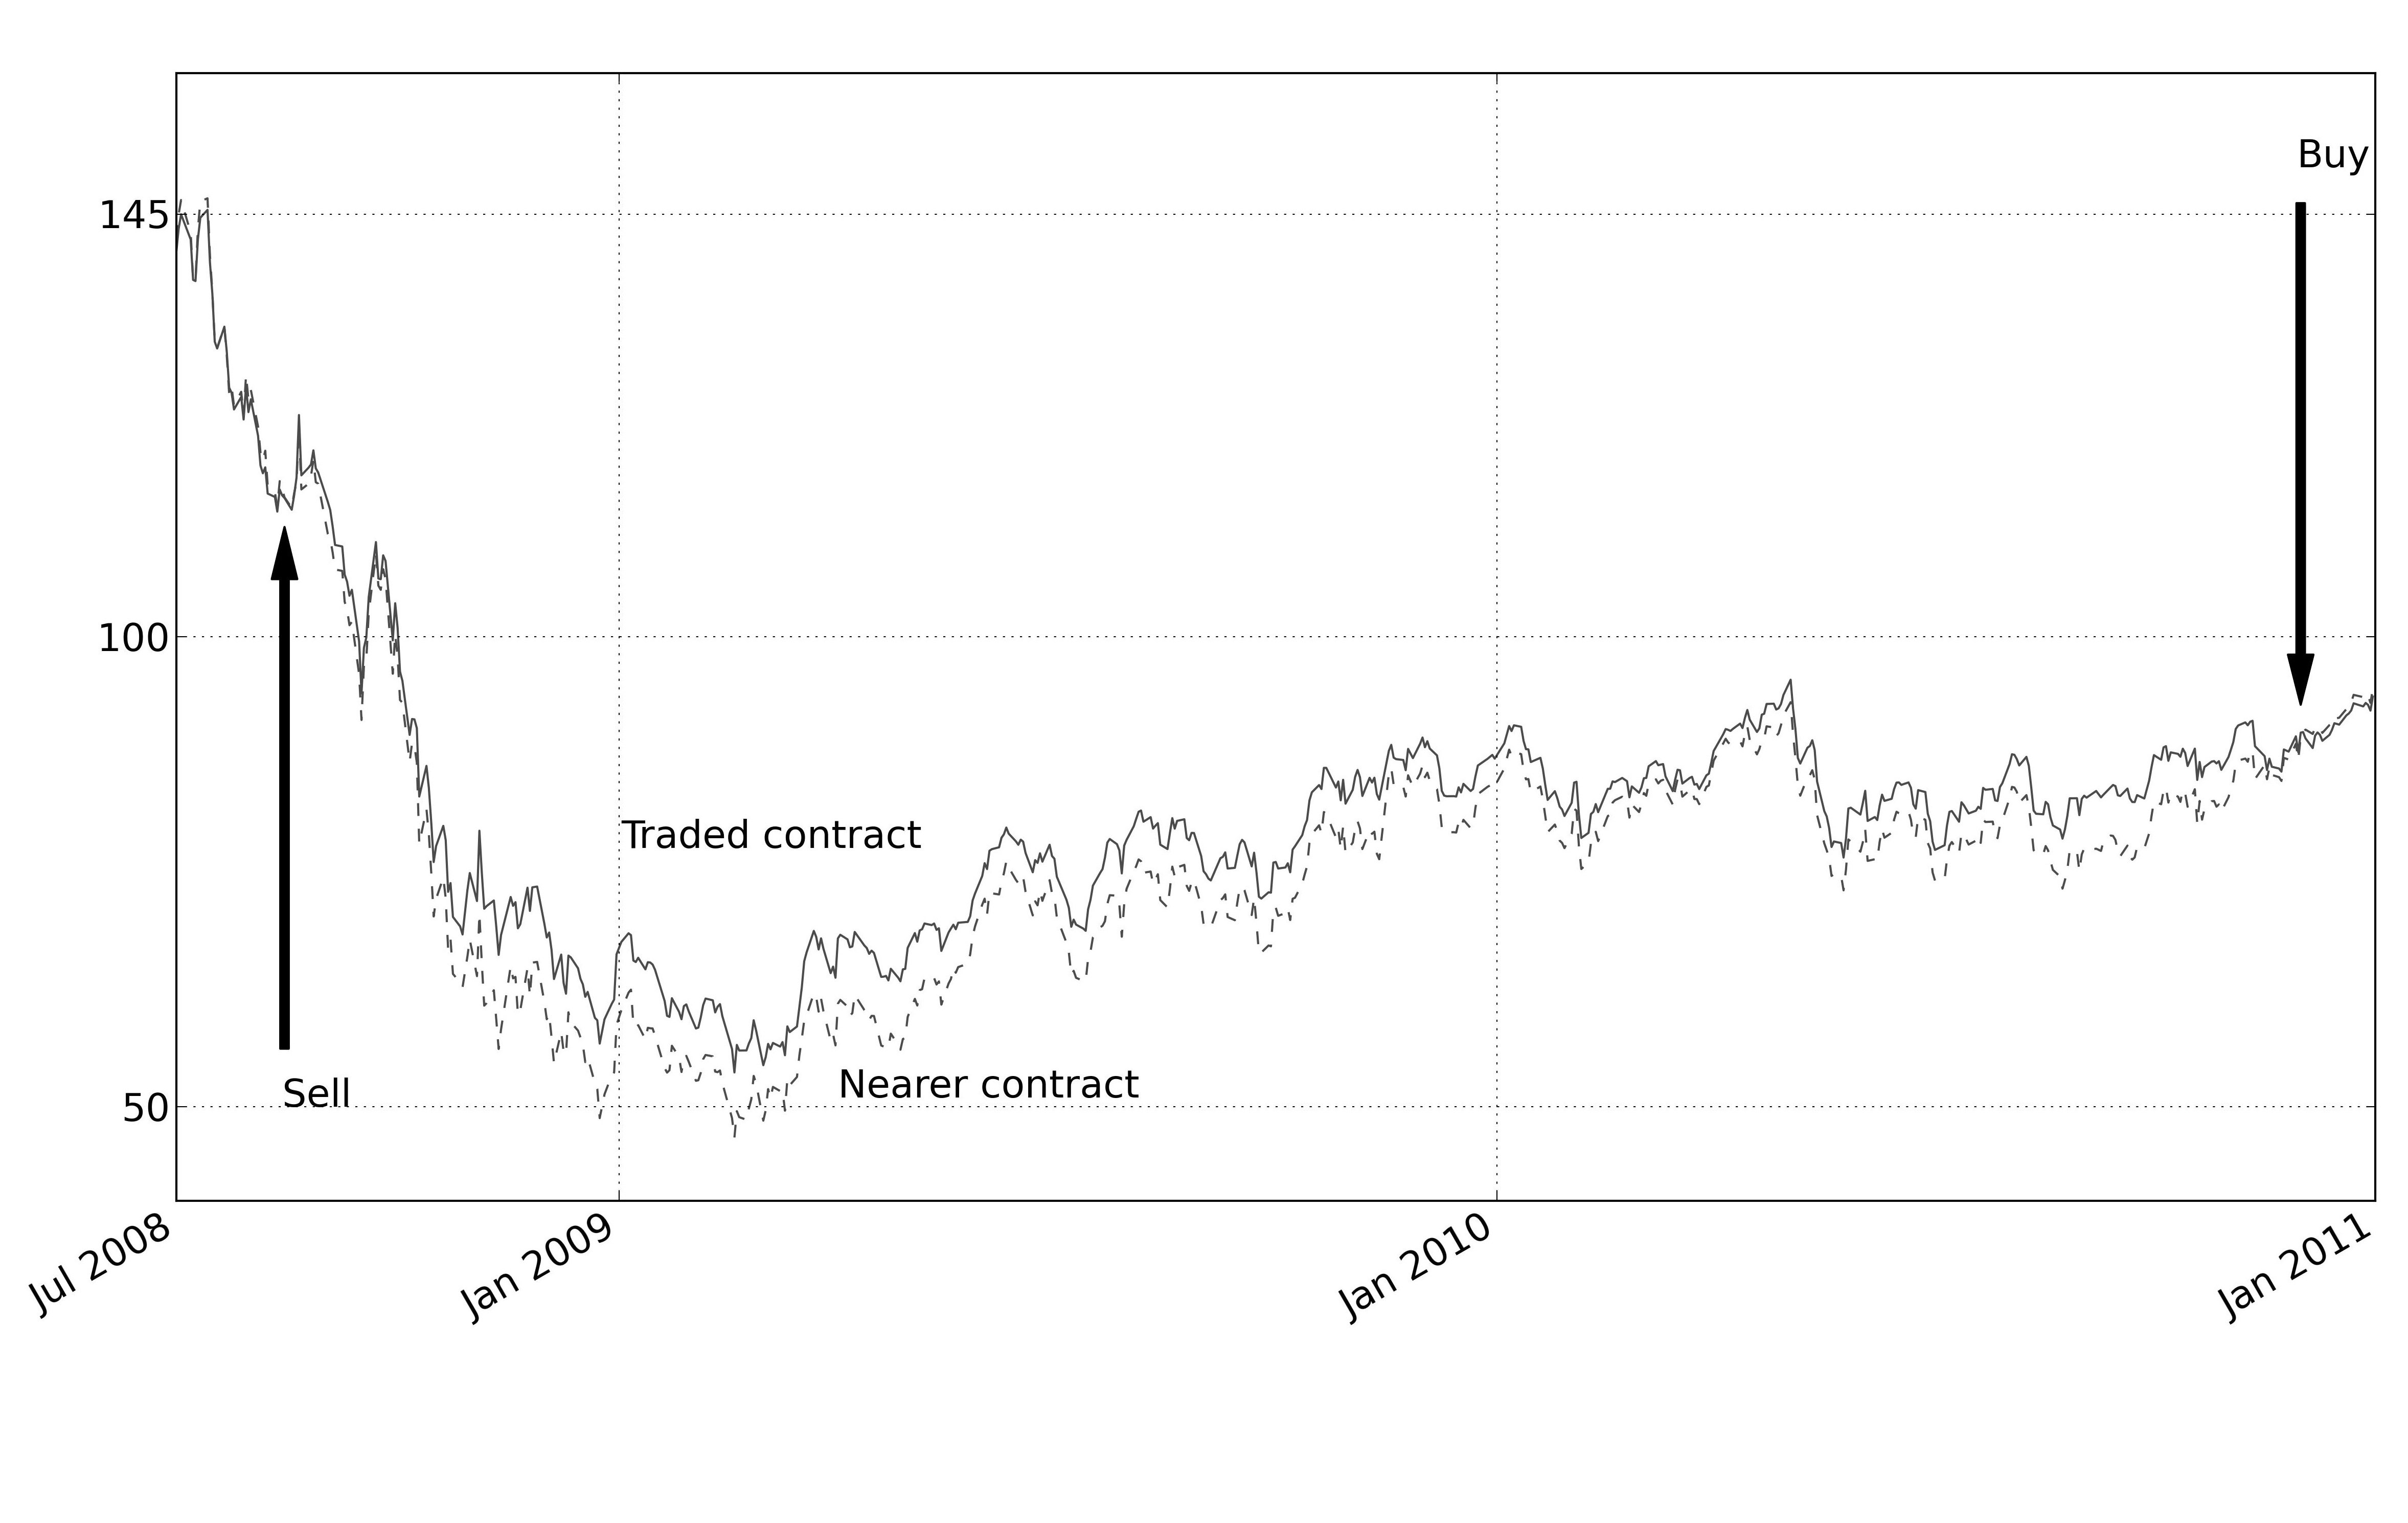
\includegraphics[width=\textwidth]{figures/raw/img-019.png} \caption{TRADING CRUDE OIL WITH CARRY IN 2008-10. WE ARE SLOW TO SELL AND STAY SHORT TOO LONG} \end{figure}

Unfortunately it remains bearish long after the market has turned, but you can't win them all. It makes sense to combine diversifying trading rules like the positive skew, trend following EWMAC rule, with a negative skew carry rule.

\section*{Adapting and creating trading rules} \phantomsection \addcontentsline{toc}{section}{Adapting and creating trading rules}

\subsection*{Staunch Systems Trader}

The above trading rules, one positive and one negative skew, are sufficient to create a pretty good trading strategy. The benefits of adding further rules within the same styles are relatively limited. Just using these two simple rules would generate roughly 85\% of the \textbf{back-tested} performance of my own more complicated system.

However you might still want to create your own rules, or adapt those you find elsewhere. Here are some pointers, with an example of how I modified a trading rule I read about whilst researching this chapter, which I've nicknamed ‘Close to Open'.

\noindent\textbf{Simplicity and objectivity.} Trading rules in books tend to be quite complicated, with lots of conditionals and a degree of subjectivity. Try and pare the rule down to its essential elements, to create a simple and objective trading rule. The example rule I found could be reduced to ‘Buy if the open is higher than yesterday's close'. (I haven't tested this rule and I have no idea if it will work or not.)

\noindent\textbf{Continuous, not binary.} Many trading rules are unfortunately of a buy or sell, binary, nature. If possible you should make them continuous. I converted the simple rule above to calculate the raw forecast as [Open price - Close price].

\noindent\textbf{Not market specific; volatility standardised.} The value of a forecast should be comparable across markets and across time. If a forecast is in price units, as in the simple example here, then you should volatility standardise it to get a forecast proportional to Sharpe ratio. So your forecast would be: [Open price - Close price ] ÷ (Recent standard deviation of daily returns). This is the same standardisation that I use in the EWMAC and Carry rules.

\noindent\textbf{Changing forecast.} Separate entry and exit rules are not suitable for the framework.* Ideally a forecast should change continuously, independently of what our position is, throughout the life of a trade. This suggests that you should create rules which recalculate forecasts every time you have new data, and then adjust your positions accordingly. Normally this is simply a matter of modifying the entry rule. Rather than use the ‘Close to Open' rule only for entries, you would calculate the forecast value every day.

\noindent\textbf{Correct scaling.} If you're going to create trading rules you need to rescale them from their natural scaling, so that the expected absolute value of the forecast is around 10. You do this by multiplying your raw forecast by a forecast scalar. You need to back-test the behaviour of the rule with real data to find the average forecast, but in line with my recommendations in chapter three, ‘Fitting', you shouldn't look at performance data whilst doing this. See appendix D, page 297, for more details. The natural average absolute value of this rule is 0.33, implying the forecast scalar in this case is 10 ÷ 0.33 = 30.

* If you absolutely have to use an entry rule which doesn't adjust throughout the life of the trade, with a separate exit rule, then I strongly suggest you use the stop loss rule I advocate for semi-automatic traders. I don't recommend using any other kind of explicit exit rule as they are usually over-fitted and make life very complicated.

\section*{Selecting trading rules and variations} \phantomsection \addcontentsline{toc}{section}{Selecting trading rules and variations}

\subsection*{Staunch Systems Trader}

Even if you don't adapt or create new rules and just use mine, there are still a theoretically infinite number of \textbf{EWMAC} \textbf{trading rule} \textbf{variations} on the menu. If you do get creative and make your own rules the number of options will explode. Which rules and variations should you use in practice? As I said in chapter three, ‘Fitting', I don't recommend using \textbf{back-tested} profitability to select trading rules or variations. Instead you should focus on behaviour such as the correlation between variations, and the speed they trade at, whilst ignoring \textbf{Sharpe ratio} and other performance metrics. You should then use two selection criteria. The first is to avoid including any two variations with more than a 95\% correlation to each other, as one of them will not be adding any value to the system. I discuss how to prune possible variations of the EWMAC rule in appendix B (in the section on EWMAC, from page 282). Secondly, you must exclude anything which trades too slowly, or too quickly. As I mentioned in chapter two, very slow rules are unlikely to generate significant Sharpe ratio.\footnote{This also means we can't prove that they work statistically.} I suggest you remove any rule which holds positions for longer than a few months. At the other end of the spectrum for many instruments fast rules will be too expensive to trade. This could mean you end up choosing a different set of variations for each instrument. I'll return to this in chapter twelve, ‘Speed and Size', where I'll show how to determine which variations should be excluded for a given level of trading costs. The \textbf{staunch systems trader} example chapter in part four will give an overview of the rule selection process.

\section*{Summary of trading rules and forecasts} \phantomsection \addcontentsline{toc}{section}{Summary of trading rules and forecasts}

\noindent{\small \setlength{\tabcolsep}{2pt} \renewcommand{\arraystretch}{1.1} \begin{tabularx}{\textwidth}{@{} p{0.24\textwidth} Y@{}}
\textbf{Where do forecasts come from} & If you're staunch systems traders then each of your trading rules produces a forecast, including any variations that we're using; for example to capture different trend lengths. Asset allocating investors use a constant identical forecast for all instruments. Semi-automatic traders make discretionary forecasts on an ad-hoc basis for a changing set of instruments. \\
\textbf{Forecast for every instrument and from each trading rule} & For staunch systems traders each instrument will have a separate forecast for a given trading rule variation. So if you had ten instruments and three different kinds of trading rule, each with two variations, then you'd calculate \(10 \times 3 \times 2 = 60\) individual forecasts. Semi-automatic traders and asset allocating investors have one forecast per instrument. \\
\textbf{Forecast sign is vital} & Positive means you buy and go long the asset. A negative forecast means you go short. A zero forecast means you shouldn't have a position. \\
\textbf{Forecast size is also important} & Absolutely larger forecasts mean you are more confident of your opinion and expect a bigger rise (or fall) in prices. Forecasts should have an expected absolute value of 10. \\
\textbf{Forecasts shouldn't be too big} & Forecasts must lie in the range -20 to +20, unless you can't short an instrument in which case it would be between 0 and +20. If a trading rule produces a larger forecast then cap it at either end of the range. \\
\textbf{Semi-automatic traders:} & Make your own predictions and convert them into forecasts between -20 (strongly bearish) and +20 (strongly bullish). Positions are closed using systematic stop loss rule, as described in chapter thirteen. \\
\textbf{Asset allocating investors:} & Use a constant forecast of +10 for all assets. \\
\textbf{Staunch systematic traders:} & Use a combination of systematic trading rules like EWMAC and Carry, design your own rule or adapt others. Follow the advice earlier in this chapter, and in chapter three, when selecting trading rule variations. \\
\end{tabularx}
}

You should now have one, or more, trading rules ready to go. \textbf{Asset allocating investors} will be using the single ‘no rule' rule, and \textbf{semi-automatic traders} will be making discretionary forecasts. If you're in either of these groups you can skip to chapter nine. Semi-automatic traders should either have developed their own rules, adapted a publically available rule, or be happy for now to use one or both of the rules I provided earlier in the chapter. If you have only one trading rule variation you can also skip the next chapter. But if you're using multiple rules or variations then you'll need to read chapter eight to discover how to combine forecasts from different rules.
